\documentclass{standalone}

%%%%%%%%%%packages%%%%%%%%%%

% \usepackage[utf8]{inputenc}

%% colors and links
\usepackage[svgnames]{xcolor}
\usepackage[colorlinks,citecolor=DarkGreen,linkcolor=DeepPink,linktocpage,unicode]{hyperref} 

%% equations
%%%% math
\usepackage{amsmath,amsfonts,amssymb,amsthm}
\usepackage{mathtools}
\usepackage{mathrsfs}
\usepackage{bm}
\usepackage{cancel}
\usepackage{dsfont}

%% positioning
\usepackage{array}
\usepackage{float}

%% table
\usepackage{booktabs}
\usepackage{multirow}
\usepackage{hhline}
\usepackage{caption}
\captionsetup{format=hang}
\usepackage{subcaption}

%% figure
\usepackage{graphicx}
\usepackage{tikz}
\usetikzlibrary{
    intersections,
    calc,
    patterns,
    through,
    positioning,
    arrows,
    backgrounds,
    decorations,
    bending,
    cd,
    tqft,
    braids,
    ext.paths.ortho,                    % for ortho paths
  ext.positioning-plus,               % for 
  ext.node-families.shapes.geometric
}
\tikzset{
    ->-/.style={
        decoration={
            markings,
            mark=at position #1 with {\arrow{>}}
        },
        postaction={decorate}
    },
    -<-/.style={
        decoration={
            markings,
            mark=at position #1 with {\arrow{<}}
        },
        postaction={decorate}
    },
    bullet/.style={
        circle,fill,
        inner sep=2pt,
        label={#1}
    },    
    process/.style={
        shape=rectangle, rounded corners, align=center, draw=#1, minimum width=0.875\linewidth, double
    },
    header node/.style={
        node family/width=header nodes,
        font=\strut\Large\ttfamily,
        text depth=+.3ex, fill=white, draw
    },
    header/.style={%
        inner ysep=+1.5em,
        append after command={
          \pgfextra{\let\TikZlastnode\tikzlastnode}
          node [header node] (header-\TikZlastnode) at (\TikZlastnode.north) {#1}
          % the next node contains both \tikzlastnode and its header
          % this is needed so that h- can be used to connect lines
          node [span=(\TikZlastnode)(header-\TikZlastnode)]
               at (fit bounding box) (h-\TikZlastnode) {}
        }
    },
    optional/.style={
        shape=diamond, align=center, draw=#1
    },
    optional process/.style={
        shape=rectangle, align=center, draw=#1
    },
}
    

\usepackage{tikz-feynman}
\usepackage{tikz-network}
\usepackage{pgfplots}
\usepgfplotslibrary{patchplots}
\pgfplotsset{compat=1.15}

%% framing
\usepackage{fancybox}
\usepackage{boites}
\usepackage{tcolorbox}
\tcbuselibrary{skins,theorems,breakable}

%%%% Japanese
\usepackage{luatexja-fontspec}
\usepackage{ascmac}
\usepackage{listings} %日本語のコメントアウトをする場合jlisting(もしくはjvlisting)が必要

%%%%%%%%%%optional settings%%%%%%%%%%


\begin{document}

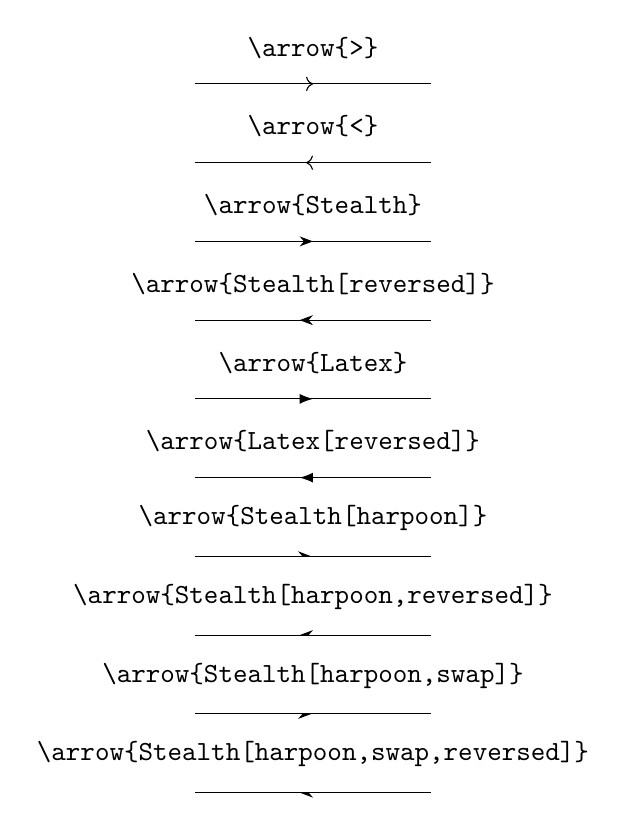
\begin{tikzpicture}
    \path foreach \i in {1,...,10} {
      coordinate (s_\i) at (0, {-\i})
      coordinate (t_\i) at (3, {-\i})
    }
    ;
    \draw[->-=.5] (s_1) -- node[midway, above=2mm] {\texttt{\textbackslash arrow\{>\}}} (t_1);
    \draw[-<-=.5] (s_2) -- node[midway, above=2mm] {\texttt{\textbackslash arrow\{<\}}} (t_2);
    \draw[
        decoration={
            markings,
            mark=at position 0.5 with {\arrow{Stealth}}
        },
        postaction={decorate}
    ] 
    (s_3) -- node[midway, above=2mm] {\texttt{\textbackslash arrow\{Stealth\}}} (t_3);
    \draw[
        decoration={
            markings,
            mark=at position 0.5 with {\arrow{Stealth[reversed]}}
        },
        postaction={decorate}
    ] 
    (s_4) -- node[midway, above=2mm] {\texttt{\textbackslash arrow\{Stealth[reversed]\}}} (t_4);
    \draw[
        decoration={
            markings,
            mark=at position 0.5 with {\arrow{Latex}}
        },
        postaction={decorate}
    ] 
    (s_5) -- node[midway, above=2mm] {\texttt{\textbackslash arrow\{Latex\}}} (t_5);
    \draw[
        decoration={
            markings,
            mark=at position 0.5 with {\arrow{Latex[reversed]}}
        },
        postaction={decorate}
    ] 
    (s_6) -- node[midway, above=2mm] {\texttt{\textbackslash arrow\{Latex[reversed]\}}} (t_6);
    \draw[
        decoration={
            markings,
            mark=at position 0.5 with {\arrow{Stealth[harpoon]}}
        },
        postaction={decorate}
    ] 
    (s_7) -- node[midway, above=2mm] {\texttt{\textbackslash arrow\{Stealth[harpoon]\}}} (t_7);
    \draw[
        decoration={
            markings,
            mark=at position 0.5 with {\arrow{Stealth[harpoon,reversed]}}
        },
        postaction={decorate}
    ] 
    (s_8) -- node[midway, above=2mm] {\texttt{\textbackslash arrow\{Stealth[harpoon,reversed]\}}} (t_8);
    \draw[
        decoration={
            markings,
            mark=at position 0.5 with {\arrow{Stealth[harpoon,swap]}}
        },
        postaction={decorate}
    ] 
    (s_9) -- node[midway, above=2mm] {\texttt{\textbackslash arrow\{Stealth[harpoon,swap]\}}} (t_9);
    \draw[
        decoration={
            markings,
            mark=at position 0.5 with {\arrow{Stealth[harpoon,swap,reversed]}}
        },
        postaction={decorate}
    ] 
    (s_10) -- node[midway, above=2mm] {\texttt{\textbackslash arrow\{Stealth[harpoon,swap,reversed]\}}} (t_10);
\end{tikzpicture}




\end{document}

